% XCircuit output "scan_main.tex" for LaTeX input from scan_main.ps
\def\putbox#1#2#3#4{\makebox[0in][l]{\makebox[#1][l]{}\raisebox{\baselineskip}[0in][0in]{\raisebox{#2}[0in][0in]{\scalebox{#3}{#4}}}}}
\def\rightbox#1{\makebox[0in][r]{#1}}
\def\centbox#1{\makebox[0in]{#1}}
\def\topbox#1{\raisebox{-0.60\baselineskip}[0in][0in]{#1}}
\def\midbox#1{\raisebox{-0.20\baselineskip}[0in][0in]{#1}}
   \scalebox{0.65}{
   \normalsize
   \parbox{6.75in}{
   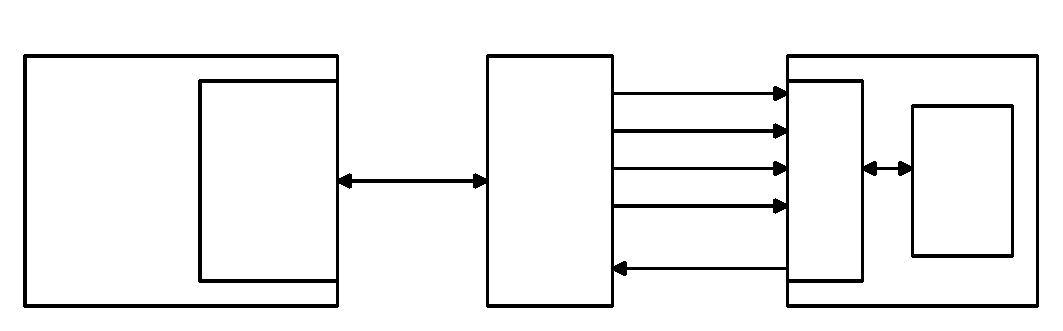
\includegraphics[scale=0.9]{scan_main.eps}\\
   % translate x=1040 y=64 scale 0.38
   \putbox{0.78in}{1.65in}{1.20}{PC}%
   \putbox{2.7in}{1.65in}{1.20}{ATxMega128}%
   \putbox{4.8in}{1.65in}{1.20}{DE0-Nano}%
   \putbox{1.23in}{0.9in}{1.20}{Python}%
   \putbox{1.28in}{0.7in}{1.20}{Script}%
   \putbox{2.02in}{0.6in}{1.20}{USB link}%
   \putbox{3.9in}{1.38in}{1.20}{{\small TDI}}%
   \putbox{3.87in}{1.15in}{1.20}{{\small TCLK}}%
   \putbox{3.9in}{0.92in}{1.20}{{\small TMS}}%
   \putbox{3.87in}{0.68in}{1.20}{{\small TRST}}%
   \putbox{3.9in}{0.11in}{1.20}{{\small TDO}}%
   \putbox{4.8in}{0.35in}{1.20}{\rotatebox{-270}{Scan Chain}}%
   \putbox{5.48in}{0.81in}{1.20}{DUT}%
   } % close 'parbox'
   } % close 'scalebox'
   \vspace{-\baselineskip} % this is not necessary, but looks better
